\documentclass[11pt,a4paper]{article}

\usepackage[margin=1in]{geometry}
\usepackage{graphicx}
\usepackage{float}

\graphicspath{{../figures/Detector_performance_analysis_Rn222_repetition_comparison/}{figures/Detector_performance_analysis_Rn222_repetition_comparison/}{figures/}{docs/figures/}{docs/figures/Detector_performance_analysis_Rn222_repetition_comparison/}}

\title{Gamma detection for source-localisation support in targeted alpha therapy}
\author{IEEE Abstract draft}
\date{}

\begin{document}
\maketitle

Targeted alpha therapies can deliver high localised dose, but treatment planning
and delivery depend on where the radionuclide source is located
after administration. Source material and progeny may remain near the
intended site, diffuse into surrounding fluid, or be redistributed by blood
flow. We evaluated whether gamma emissions from the
Rn-222 decay chain could provide source-location information by simulating
Rn-222 activity within a loaded cyanoacrylate layer, attached to a water phantom
and surrounded by six detector panels. Six source configurations were
compared: one retained-source baseline, three diffuse-water cases with 10\%,
50\%, or 90\% of activity placed in the water volume, and two localized
water-displacement cases with 40\% or 60\% of activity placed in a displaced
region. Each configuration used ten repetitions of 10,000
primary Rn-222 events. Each photon entry into a detector panel was counted
as one hit. Overall detector hit rate shifted only slightly, from
1.250 $\pm$ 0.008 hits per primary event for the retained-source baseline
to 1.206 $\pm$ 0.009 for the 90\% diffuse-water case. In contrast, panel
balance and spatial profiles changed substantially: activity displaced from
the loaded layer reduced the dominant positive-y response and increased the
negative-y, lateral, and longitudinal detector responses. Profiles corrected by baseline subtraction revealed these source-specific residuals. The signal was visible on
hour-scale cumulative windows, with baseline simulations yielding about 106
detector hits by 2 hours and 978 by 12 hours per 10,000 primaries, and
became stronger over longer windows, reaching about 3639 hits by 2 days
and 7218 by 5 days. The \(t<10^6\) s cut suppresses the late Bi-210 tail.
These results indicate that gamma detection from Rn-222
progeny may provide source-location information not captured by total count
rate alone, supporting treatment planning, delivery verification, and
adaptive assessment in targeted alpha therapy.

\newpage

\section*{Alternative Version with figures}
\section*{Gamma detection for source-localisation support in targeted alpha therapy}
Targeted alpha therapies can deliver high localised dose, but treatment planning
and delivery outcome depend on where the radionuclide source is actually located
after administration. Source material and progeny may remain near the intended deposition
site, diffuse into surrounding fluid, or be redistributed by biological
transport such as blood flow. We evaluated whether gamma emissions from the
Rn-222 decay chain could provide source-location information by simulating
Rn-222 activity within a loaded cyanoacrylate layer, attached to a water phantom
and surrounded by six photon-detector panels. Six source configurations were
compared: one retained-source baseline, three diffuse-water cases with 10\%,
50\%, or 90\% of activity placed in the water volume, and two localized
water-displacement cases with 40\% or 60\% of activity placed in a displaced
region. Each photon entry into a detector panel was counted as one hit, and
detector-panel hit counts and spatial profiles were compared by
subtracting the retained-source baseline.

\begin{figure}[H]
\centering
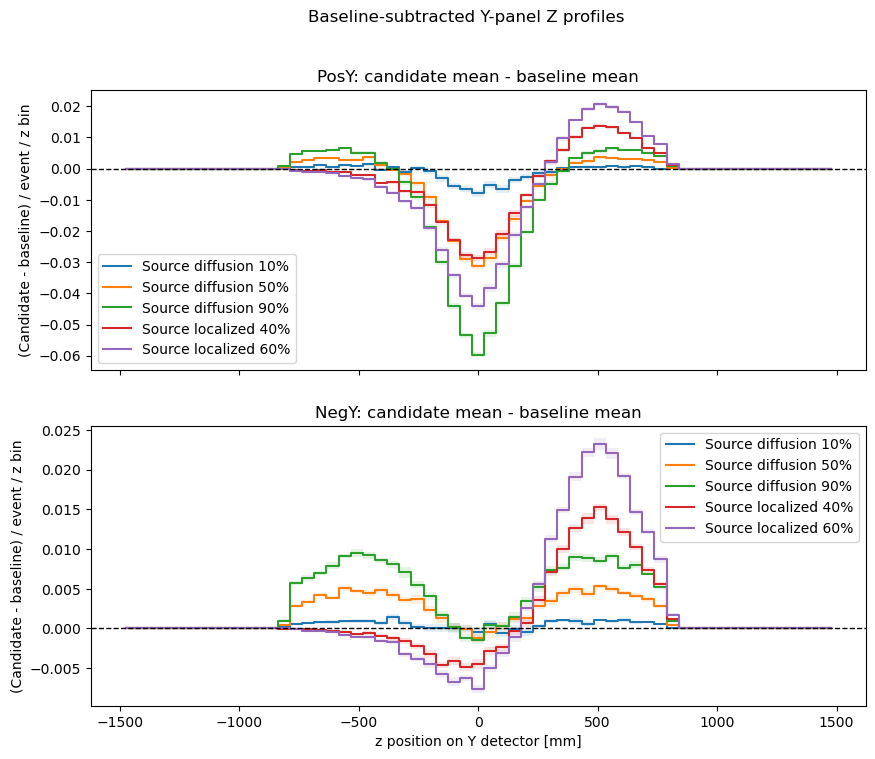
\includegraphics[width=0.82\textwidth]{y_panel_baseline_subtracted_z_profiles.png}
\caption{Baseline-subtracted detector-hit profiles for the positive- and
negative-\(y\) panels. Source movement changes the spatial distribution of
detected gamma events, not only the total count rate.}
\label{fig:abstract-y-profile}
\end{figure}

Overall detector hit rate shifted only slightly, from 1.250 $\pm$ 0.008
hits per primary event for the retained-source baseline to 1.206 $\pm$
0.009 for the 90\% diffuse-water case. In contrast, panel balance and
spatial profiles changed substantially: activity displaced from the loaded
layer reduced the dominant positive-\(y\) response and increased the
negative-\(y\), lateral, and longitudinal detector responses.
Profiles corrected by baseline subtraction revealed these source-specific residuals.
\begin{figure}[H]
\centering
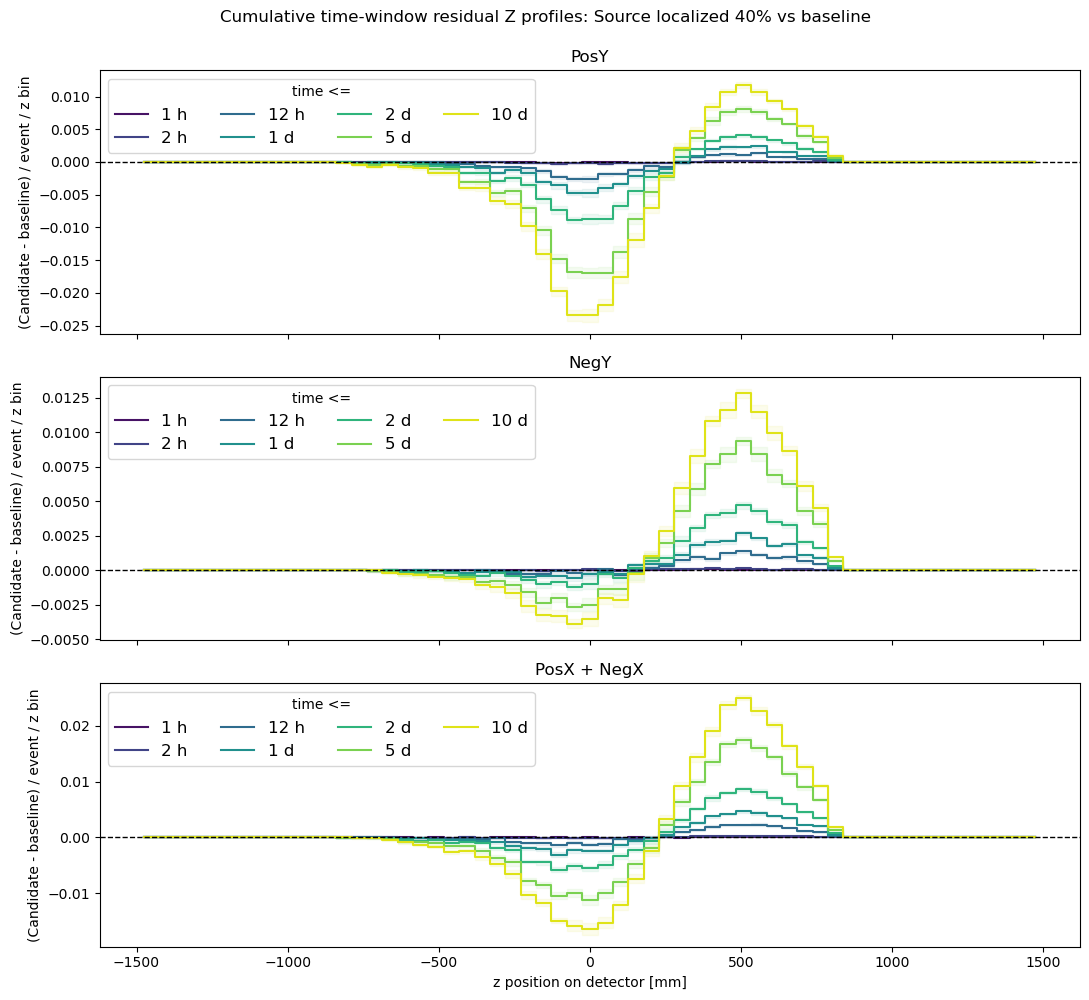
\includegraphics[width=0.82\textwidth]{time_window_residual_z_profiles_loc40.png}
\caption{Cumulative time-window residual profiles for the localized
source-displacement case with 40\% of activity in the localized water
region. The baseline-subtracted signal is visible within hours and becomes
stronger over multi-day windows.}
\label{fig:abstract-time-profile}
\end{figure}

The signal was visible on hour-scale cumulative windows, with baseline
simulations yielding about 106 detector hits by 2 hours and 978 by
12 hours per 10,000 primaries, and became stronger over longer windows,
reaching about 3639 hits by 2 days and 7218 by 5 days. A \(t<10^6\) s
analysis window retains the Po-214/Bi-214 signal while excluding the later
Bi-210 tail. These results
indicate that gamma detection from Rn-222 progeny may provide
source-location information not captured by total count rate alone,
supporting treatment planning, delivery verification, and adaptive
assessment in targeted alpha therapy.

\end{document}
